\documentclass[letter]{article}

\usepackage[english]{babel}
\usepackage[utf8]{inputenc}
\usepackage{amsmath}
\usepackage{graphicx}
\usepackage[colorinlistoftodos]{todonotes}
\usepackage[citestyle=alphabetic, maxbibnames=99, sorting=ydnt]{biblatex}
\usepackage[stable]{footmisc}
\usepackage{tikz}
\usetikzlibrary{plotmarks}

\newcommand{\sys}{\textit{Speedy}\space}

\addbibresource{literature.bib}

\usepackage{fontspec}

\title{\sys\!: a Sybil-resistant DHT implementation\footnote{https://www.github.com/wzheng/speedy}}

\author{Quanquan Liu, Qian Long, Pratiksha Thaker, Wenting Zheng}

\date{\today}

\begin{document}
\maketitle

\section{Introduction}

Distributed hash tables (DHTs) are common services that leverage peer-to-peer
(P2P) communication to provide a distributed key value service across nodes in a
network. The tasks of nodes in a distributed hash table include storing
key/value pairs and providing values for lookup requests or rerouting requests
to other nodes. A public DHT should be able to handle nodes joining and leaving
arbitrarily, and provide efficient lookups, key inserts, and value
modifications.

A classic vulnerability in such a network is a \textit{Sybil attack}, in
which a an adversary is able to introduce malicious nodes, which
do not adhere to specified
protocols, into a network . Specifically,
by introducing a large number of these malicious nodes with fake identities,
the adversary is able to
disrupt system operation by responding to queries with incorrect information;
maintaining an incorrect routing table, delaying queries;
strategically placing nodes in an attempt to construct a snapshot of the
entire network's data, possibly subverting security properties; or a
number of other potential attacks.

In this project, we designed and implemented a DHT to mitigate some
Sybil attacks and provide data consistency, while minimizing the number of hops
for a lookup, given certain assumptions about the underlying P2P network.
Our implementation is based on the \textit{Wh\={a}nau} routing protocol
\cite{whanau}, but includes a layer of indirection to allow key operations
to be coordinated using Paxos, as well as basic key signing to provide
data integrity.

\section{Related work}

Past projects including SybilGuard \cite{sybilguard}, SybilLimit \cite{sybillimit},
and Wh\={a}nau \cite{whanau} have examined this problem in the context
of fast-mixing social networks, with specific restrictions on the
structure of the resulting graph. This work primarily addresses attacks
in which malicious nodes delay or re-route queries; data integrity
problems are assumed to be handled by the client via signatures or another
verification measure.\\

As in previous work, we assume that the underlying graph is a social network.
As shown in \cite{whanau}, this allows us to assume the honest region is
fast-mixing and, assuming that creation of a link between honest and Sybil
nodes is difficult, there exists a sparse cut between the honest region
and the Sybil region.


\section{Design}

We separate our design into two "layers": the routing layer, based on
\cite{whanau}, and the consistency layer, composed of multiple clusters of
servers which coordinate key operations using Paxos.

\subsection{Routing protocol}
For the routing part, we use the original Wh\={a}nau protocol as presented in \cite{whanau}. In this "layer", each key is matched with list of nodes that comprises of the Paxos cluster responsible for that key. In our design, we call these key/value pairs, where value is a list of server names. The true value of the key is replicated across the nodes in the paxos cluster, which is explained in the next section. The routing protocol is responsible for retrieving the Paxos cluster assigned to a key, which we will refer to as the "value" for the remainder of this subsection.

The Wh\={a}nau protocol relies heavily on random walks and random sampling to build up its routing tables.
Because of the sparse cut assumption in our network model
and the fast mixing properties of the honest node region,
random walks from any node are likely to stay within the honest region
unless the node is part of the sybil edges.

Each node maintains a local key/value store for the keys that are inserted from this node. Each key in the local kv store will get assigned a Paxos cluster value as explained in secton 3.3.
After this assignment, each node creates an intermediate key/value store, called db, that contains $r_d$ samples of key/value pairs collected from random walks on the network.
The Wh\={a}nau protocol introduces the idea of layers of routing tables provably useful for mitigating some Sybil attacks \cite{whanau}.

In each layer, there are three routing tables created: id, fingers, successors.
The id for a layer is used to identify the node; it comes from the keyspace. This is chosen randomly from the db for the first layer and chosen randomly from the previous layer's fingers in subsequent layers.
The fingers contains $r_{f}$ (id, server) pairs that act as pointers to other nodes in the network for routing. The fingers are chosen from taking random walks on network.
The successors contains records that follow the id in the keyspace. The successors are built up by taking $r_{s}$ random walks and collecting the records close to the current layer's id from each of the random walks.

The routing table setup outlined above builds a static routing table on each node in the network with sybil attack resistant properties explained in \cite{whanau}. In order to account for new inserts into the DHT, this routing table setup must happen periodically so that the DHT can be up-to-date.

\subsection{Replication and consistency}

The Wh\={a}nau protocol naturally results in a large amount of replication,
but does not specify consistency guarantees or a protocol for key inserts
and value updates. \sys trades this large amount of replication for
stronger consistency guarantees by creating Paxos clusters within
the DHT which store the values for each key, rather than storing them
in the Wh\={a}nau routing tables. This gives us two advantages: first,
very large data values will not be excessively replicated, which would
otherwise use up large amounts of storage space; second, concurrent
updates and node failures are resolved through the master clusters, which will be
explained in section 3.6.

The Paxos cluster for each node is chosen by using random walks. Given user defined
${PaxosSize}$, \sys uses ${PaxosSize-1}$ random walks to construct the Paxos cluster.
Each server's paxos cluster is constructed during the $SETUP$ stage. Each server,
once it enters the set up stage, will perform random walks in order to find $PaxosSize-1$
servers. The server then starts a two phase commit with those nodes in order to form
the Paxos cluster.

\subsection{Setup}
Because the routing tables created in the Whanau Protocol are static, the setup steps must happen periodically to account for key churn and node churn in the network.

Setup works as follows for one node
\begin{enumerate}
\item For every key in a node's queue, ask the Master cluster to assign a Paxos cluster for it. This populates the local kvstore.
\item Build up routing tables using the Whanau Protocol
\end{enumerate}

\subsection{Lookup}
The following outlines a lookup for key $k$.
\begin{enumerate}
\item Look in local kv store to find the Paxos cluster for $k$, if not found, follow the steps below to look for it.
\item Randomly choose a layer, and randomly choose a finger, $n_{f}$ in that layer close to the key.
\item Look in the successors of $n_{f}$.
\item Repeat steps 2 and 3 until found or time out. The high level of replication in the protocol ensures that it will usually take 1 hop to find the Paxos cluster of a key.
\item Now that we have the Paxos cluster of $k$, we use the Paxos protocol within the nodes in the cluster to agree on the true value to return to the client.


\end{enumerate}

\subsection{Dynamic updates}

Storing true values in Paxos clusters naturally allows support for dynamic value
updates: a Put operation is simply routed to the appropriate cluster, and the
servers involved come to a consensus on the ordering of the operation in their
logs. This also addresses the potential concern of two different clients
attempting to update the value of the same key concurrently. In this way,
clients need not wait for a Setup round to see the effect of their value
operations.

\subsection{Dynamic inserts}

Inserting new keys is slightly more involved than value updates, as the
construction of routing tables in Wh\={a}nau depends on knowledge of the existing
keys in the network. To address this, we assign a certain set of servers to be
"master" servers, which also coordinate operations using Paxos. These master servers
are pre-determined before the very first setup, and therefore do not change in the
later setup stages. All of the servers in the DHT know of these master servers. When
an insert happens, it becomes a pending insert. This has to happen because Wh\={a}nau
cannot handle new inserts until a new setup is run. Therefore, each server processes
these new inserts by sending that information to a random master node. The master
node is in charge of initiating a paxos call to the other master servers and decide
on which server to send the pending insert.

After the master servers agree on a key-server mapping, all subsequent pending
inserts will always be sent to that server. This Paxos operation takes care of
concurrent inserts to the same key by multiple servers. Note that one master server
could solve the problem, but we have multiple master servers in order to make
\sys more tolerant. Also note that masters are only used for insert operations, and
only have limited powers.

\subsection{Fault tolerance}

Wh\={a}nau provides fault tolerance through large amounts of replication. Our
implementation maintains this at the routing layer, but the fault tolerance
properties at the data layer are somewhat less obvious; we informally
discuss them here.

%%% TODO why actually
We use $O(\log n)$ replicas in each Paxos cluster, each selected by a random walk
of length $O(\log n)$, in order to ensure that each cluster has a constant
number of honest nodes, where $n$ is the total number of honest nodes in the
DHT \cite{whanauthesis}. Each Paxos cluster is responsible for one key;
the clusters are constructed and the keys assigned at Setup time.
If a node fails, it can no longer participate in consensus in any Paxos
cluster it is a part of. However, even correlated node failures will
not result in correlated Paxos failures; since clusters are created using
random walks, the effects of node failures will be "distributed" over
many Paxos clusters.

Fault tolerance in the routing layer (in particular, the effects of
Sybil nodes which may re-route queries) is the same as described in
\cite{whanau}.

\subsection{Data Integrity}
In addition to fault tolerance and consistency, \sys also provides some data integrity guarantees. In a public DHT, Sybil nodes could constantly update
new values for existing keys. There is no good way to know whether a particular
put operation inserted an ``incorrect'' value because we cannot tell whether
a node is malicious or not. We can only provide a guarantee that a particular
value will always be tracked back to the node that executed that put operation.
This information could then be used in a reputation system for this public DHT.
The reputation system is outside the scope of this project, so we will only
provide an explanation for a method for ensuring data integrity.

In our data integrity model,
each node in the network has a secret key and public key. We refer to the originator as the node who performs the put request. When a \texttt{(key, true value)} is inserted, the originator signs a concatenation of \texttt{(true value || originator ip address || originator public key)} with its secret key.
The originator then concatenates the true value, originator ip address, signature, and his public together as the new true value of the key.
If a node does not include all of the valid information, then its put request will be rejected.

During a lookup, after the true value is retrieved from a Paxos cluster, the receiving node can verify the integrity of the data by verifying the signature with the attached public key.

Note that this scheme does not provide any confidentiality because the original value
is always stored in plain text. Therefore, a malicious node can always take someone else's value and sign with its own secret key. Information requiring confidentiality should be
encrypted using public key encryption, and it should be taken care of on the client side.

Sybil nodes could potentially try to imitate an honest node by signing with its secret key,
but then say that the information came from an honest node's IP. This problem can be solved by
requiring the originator IP address to be included in the true value so that any node can ask the originator for its public key to check with the one that is attached.

Of course, sybil nodes can still coordinate with each other to verify each others public keys. In this case, we can build a reputation system to keep track of suspicious nodes. For example, if the data received is a virus, then that ip address/public key pair will get a low ranking in the reputation system. More research is needed in this area, but we believe that our scheme is a good start for providing some basic data integrity in \sys.

\section{Performance}

\subsection{Setup: systolic mixing}

A bottleneck in our implementation was the overhead in sending out many random
walks throughout the Setup process. To mitigate this, we implemented the "systolic
mixing" process suggested in \cite{whanauthesis}, in which random walks are
precomputed by flooding the network with node addresses and shuffling them at each
time step. This reduced the time for Setup with large numbers of servers (over 100)
to less than 10\% of the time it took using recursive random walks.

\subsection{Whanau Lookup hop count}
The Whanau Protocol guarantees a one hop lookup with high probability \cite{whanau}. Recall in \sys, the whanau lookup is the first part of the protocol where we look up the Paxos cluster responsible for a key. One hop means that we do steps 2 and 3 of the Lookup Protocol (3.4) from the node issuing the request. If that fails, we hop to another node (via random walk) and try again.


We tested this claim experimentally using a 100 node network that is well connected and 5 pre-inserted key/value(Paxos cluster list) pairs per node, giving a total of 500 keys in the network.

After one setup phase, we performed the Whanau Lookup from every node on every key and count the number of hops in each Whanau lookup. This is $100 \cdot 500$ lookups in total. Results from 5 trials show that an average of .5 percent of all the Whanau Lookups required more than 1 hop. This shows good empirical evidence for the 1 hop lookup claim.

Furthermore, we test the claim on different network structures to observe the effect. We construct network graphs where each node has a probability $P$ of being neighbors with any other node in the network. $P$ is referred to as the edge probability in the table below. Once again, we use a 100 node network of honest nodes with 500 total key/value pairs. We see
that the one-hop lookup claim holds up to small numbers of
edges, at which point the number of lookups requiring more than one
hop increases slightly but is still quite low.\\

\begin{center}
\begin{tabular}{| l | l | l |}
\hline
Edge Prob & Fraction of Successful Lookups needed > 1 Hop & Total Lookup Success\\ \hline
1.0 & 0.004 & 1.0\\ \hline
0.9 & 0.006 & 0.99\\ \hline
0.8 & 0.003 & 1.0\\ \hline
0.7 & 0.004 & 1.0\\ \hline
0.6 & 0.0019 & 1.0\\ \hline
0.5 & 0.005 & 1.0\\ \hline
0.4 & 0.007 & 1.0\\ \hline
0.3 & 0.0037 & 1.0\\ \hline
0.2 & 0.004 & .998\\ \hline
0.1 & .0094 & .998\\ \hline
\end{tabular}
\end{center}

\section{Security Analysis}

\subsection{Thread Model}
The "Sybil Proof" security of \sys is based upon the assumption that there is a sparse cut between the fast mixing honest region and the Sybil region of the underlying p2p network. There are no further assumptions on the graph structure of the Sybil region. The routing tables and Paxos clusters are all built up from taking random walks on the network. The main intuition is that a random walk from an honest region is unlikely to end up in the Sybil region because of the sparse cut, unless, of course that honest node is on the edge of the graph.

Besides the sparse cut assumption, Sybil nodes are free to behave however they wish. This can include dropping routing packets, flooding the neighbors, clustering attacks, modifying data values from within the DHT, blatantly returning wrong values, etc.

The main security guarantee \sys provides is that Lookups return correct values most of the time even in the presence of a majority of Sybil nodes. This is based on the security guarantees of Whanau shown in \cite{whanau}. Though we extended the protocol with a layer of indirection for providing data consistency, we believe the security guarantees should still be valid.

The security analysis of \sys can be broken down into the security of the routing layer (looking up the Paxos cluster for a particular key) and the security of the data layer (looking up the true value from the Paxos cluster). We explain some of the theoretical guarantees and show experimental results.

% Include experimental results and pretty charts here that take up lots of space =D
\subsection{Whanau Routing Layer Security}
The main security guarantee in the routing layer of the protocol is that Whanau Lookups are successful most of the time in the presence of a large number of Sybil nodes. We tested this on multiple graphs of different numbers of well-connected graphs (with respect to honest nodes), numbers of Sybil nodes, and number of keys. The first simulation was run on a graph with $50$ honest nodes, $50$ Sybil nodes, and a maximum of $5$ keys per node. The simulation with varying number of attack edges randomly and approximately uniformly dispersed throughout the honest nodes. It tested lookups of all the keys that are in honest nodes from every honest node and computed the fraction of these lookups that are successful. The results of the simulation can be seen in Figure~\ref{fig:sybilattackedges}. 

\begin{figure}[!h]
\centering
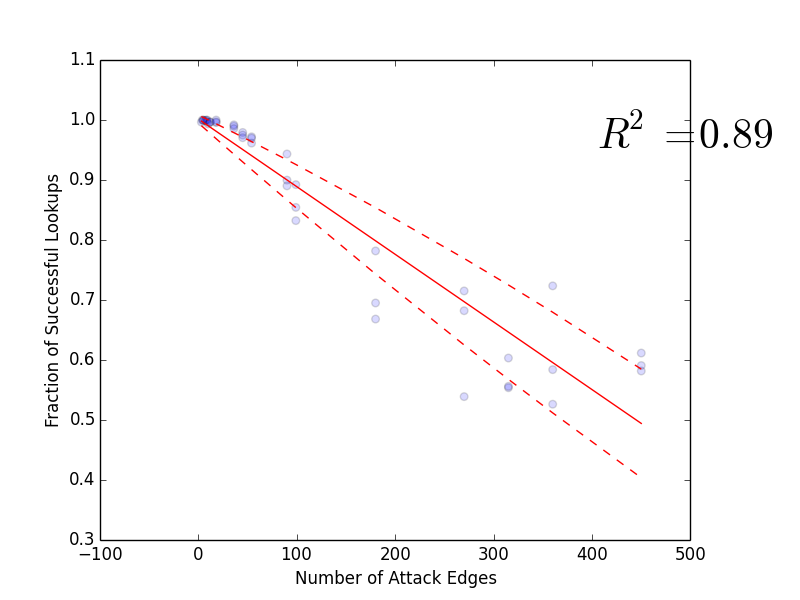
\includegraphics[width=0.9\columnwidth]{sybilattackedges}
\caption{Number of attack edges in a graph with $50$ honest nodes, $50$ Sybil nodes, and $5$ keys per node. Each honest node is connected to every other honest node. Each Sybil node is connected to every other Sybil node. With a certain probability an edge is determined to exist between an honest and Sybil node. The probability varies among different runs of the simulation. The fractions of successful lookups decreases as the number of attack edges increase. However, the protocol does fairly well reaching approximate $50\%$ success for $450$ attack edges (approximately $1/3$ the number of edges between honest nodes).}
\label{fig:sybilattackedges}
\end{figure}

Fig.~\ref{fig:sybilattackedges} shows that the fraction of successful lookups dropped off slowly reaching $50\%$ success with $450$ attack edges, which is $1/3$ of the total number of edges between honest nodes. We also varied the number of Sybil nodes present in the graph. For the second simulation, we created $70$ honest nodes, $30$ Sybil nodes, and $5$ keys per node. The results of this simulation can be seen in Fig.~\ref{fig:sybilattackedges30}.

\begin{figure}[!h]
\centering
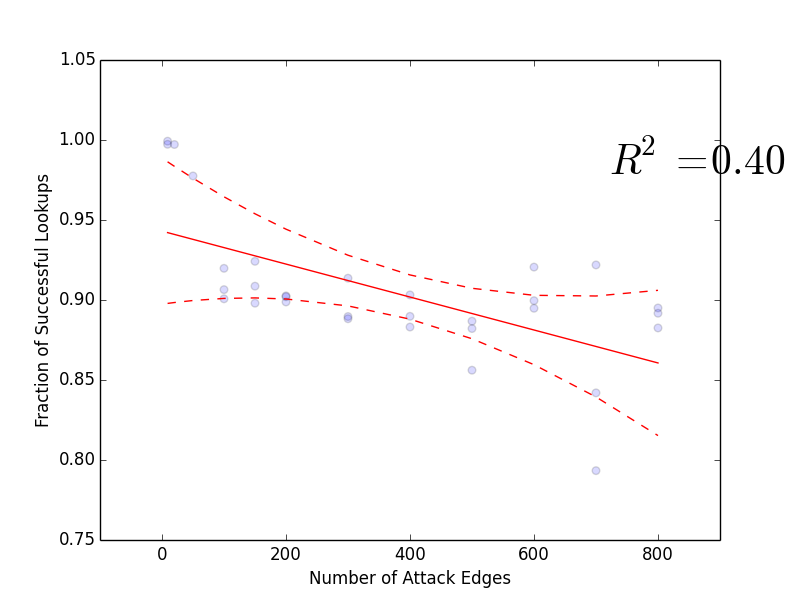
\includegraphics[width=0.9\columnwidth]{sybilattackedges30}
\caption{Number of attack edges in a graph with $70$ honest nodes, $30$ Sybil nodes, and $5$ keys per node. The protocol has a fraction of success of approximate $88\%$ for $800$ attack edges (again approximately $1/3$ the number of edges between honest nodes).}
\label{fig:sybilattackedges30}
\end{figure}

We see that the \emph{number} of Sybil nodes does affect the fraction of successful lookups. This is a surprising result because we expected to see that the fraction of successful lookups depend more on the number of honest nodes and the number of attack edges between honest nodes and Sybil nodes. In other words, a larger number of honest nodes leads to more edges between honest nodes, thus leading to a higher threshold for the number of attack edges that can be tolerated before the number of successful lookups decreases significantly. However, Fig.~\ref{fig:sybilattackedges30} shows that despite having $800$ attack edges ($1/3$ of the number of honest edges), the fraction of success still hovers around $88\%$. We are not quite sure why this occurs but one explanation could be that the number of potential Sybil clusters that could occur decreases as the number of Sybil nodes decreases.

\subsubsection{Sparse Cut Assumption Relaxed}

\subsubsection{Clustering Attack}

\subsection{Data Layer Security}

\subsubsection{Paxos Security}
While paxos security on the Paxos protocol level is out of the scope of this project, we
\section{Future work}

We have implemented the Whanau protocol as it is described in
\cite{whanauthesis}, including a layer of indirection to provide
data consistency as well as a layer of key signing to provide
data integrity. However, our implementation requires a set of master
nodes, which could turn into a bottleneck and increase latency
significantly; future work might involve distributing the work of the
master nodes further.

We would also like to do correctness and integrity testing on a much
larger scale to determine how many node failures our system can tolerate.
Furthermore, we have not yet tested our system with significant changes
to the graph structure in between Setup phases, although we believe
we have increased its robustness to such changes by adding Paxos logging
so that nodes leaving the network nevertheless allow the remaining
nodes to agree on operations.

\printbibliography
\nocite{*}

\end{document}
